% $Header$

\documentclass[aspectratio=1610]{beamer}

\mode<presentation>
{%
  \usetheme{Boadilla}
}


\usepackage[english]{babel}
\usepackage[utf8]{inputenc}
\usepackage[T1]{fontenc}

\usepackage{%
    animate,
    graphicx,
    varwidth,
    tcolorbox,
    clrscode3e,
    tikz,
    mathtools,
}
\usetikzlibrary{shapes.multipart}

\tikzset{%
    block/.style={%
        font=\sffamily,
        draw=black,
        thin,
        fill=pink!50,
        rectangle split,
        rectangle split horizontal,
        rectangle split parts=#1,
        outer sep=0pt
    },
    gblock/.style={%
        block,
        rectangle split parts=#1,
        fill=green!30
    },
    invisible/.style={opacity=0},
    visible on/.style={alt={#1{}{invisible}}},
    alt/.code args={<#1>#2#3}{%
      \alt<#1>{\pgfkeysalso{#2}}{\pgfkeysalso{#3}} % \pgfkeysalso doesn't change the path
    },
}

\graphicspath{{../../imgs/}}

% alert a whole line (especially for algorithms)
\newcommand{\alertline}{%
 \usebeamercolor[fg]{normal text}%
 \only{\usebeamercolor[fg]{alerted text}}}

% floor command
\newcommand{\floor}[1]{\left\lfloor #1 \right\rfloor}

\title[ALG25 - Lecture 4]
{Elemental Datastructures, Heaps and Priority Queues}

\subtitle
{Algorithms and Datastructures, F25, Lecture 4}

\author[Andreas H. Høeg-Petersen]
{Andreas Holck Høeg-Petersen}

\institute[AAU]{%
  Department of Computer Science\\
  Aalborg University
}

\date {\today}

\pgfdeclareimage[height=0.5cm]{university-logo}{../../imgs/aau-logo}
\logo{%
    \begin{tikzpicture}[overlay,remember picture]
        \node[left=0.2cm] at (current page.30){\pgfuseimage{university-logo}};
    \end{tikzpicture}
}

\AtBeginSection[]
{%
  \begin{frame}<beamer>{Outline}
    \tableofcontents[currentsection,currentsubsection]
  \end{frame}
}


\begin{document}

\begin{frame}
  \titlepage
\end{frame}

\begin{frame}{Opdateringer}{}
    \begin{itemize}[<+->]
        \small
        \item Programmeringsopgave 1 --- godt arbejde! Hvorfor var quicksort
            langsom for de store, random lister?
        \item Fra evaluering:
            \begin{itemize}
                \item 20 svar sidst - fedt!
                \item Flere ønsker mere tid til opgaver
                    \begin{itemize}
                        \item Svært at gøre noget ved, da vi ikke har mere tid
                        \item Opgavesættene er ikke nødvendigvis designet til at
                            kunne laves på 2 timer (dvs: hjemmearbejde nok
                            nødvendigt, hvis man vil igennem dem!)
                        \item Vi kunne godt skrue ned på tiden brugt i
                            forelæsningerne på at gennemgå algoritmerne, men\ldots
                    \end{itemize}
                \item Flere mente tiden var godt fordelt mellem opgaver og
                    forelæsning
                    \begin{itemize}
                        \item Der var også flere, der eksplicit var glade for
                            den tid, vi bruger på at gennemgå eksempler og
                            algoritmer
                    \end{itemize}
                \item `Svært at holde fokus i del 2' + `Fik ikke særligt meget
                    at spise og drikke'
                    \begin{itemize}
                        \item Del 2 \alert{vil være tungere} pga tidspunktet
                        \item Bedste løsning: få noget ordentligt at spise og
                            drikke og husk at passe jeres søvn <3 
                    \end{itemize}
            \end{itemize}
    \end{itemize}
\end{frame}


\begin{frame}{Outline}
  \tableofcontents
\end{frame}


\section{Elementære datastrukturer}


\begin{frame}{Datastrukturer}{Hvad og hvorfor?}
    En datastruktur er i bund og grund blot en \alert{struktureret} samling af
    \alert{data}. \pause

    \begin{itemize}[<+->]
        \item I kender allerede \alert{arrays}, som er en sekvens af
            data-elementer af en bestemt type startende fra index 0 (eller 1,
            hvis man er CLRS-bogen\ldots)
        \item Vi benytter arrays som den fundamentale byggesten til at
            konstruere \alert{dynamiske mængder} (`sets')
        \item Dynamiske mængder er noget, vi kan manipulere, f.eks.\ via
            \proc{Insert}, \proc{Delete}, \proc{Search} eller lignende
            operationer
        \item Vi starter med at kigge på \alert{stacks} og \alert{queues}, som
            følger to forskellige principper for \proc{Insert} og \proc{Delete}
    \end{itemize}
\end{frame}

\begin{frame}{Stacks}{Last in, first out}
    En helt fundamental datastruktur er \alert{stakken} (en `stack'). Den kan
    bedst sammenlignes med en stak tallerkener og følger
    \alert{LIFO}-princippet: `Last In, First Out'.

    \begin{columns}
        \column{.5\textwidth}
        \begin{itemize}
            \item Insertion og deletion kaldes henholdsvis \alert{Push} og
                \alert{Pop}
            \item Vi implementerer en stack med plads til $n$ elementer med et
                array $S[1\ldots n]$
            \item Vi definerer en attribut $\attrib{S}{top}$, der peger på det
                index i $S$, hvor det seneste indsatte element befinder sig
            \item $\attrib{S}{size}$ fortæller os hvor stor stacken er (dvs.\ $n$)
        \end{itemize}
    
        \column{.5\textwidth}

        \begin{figure}[h]
            \centering
            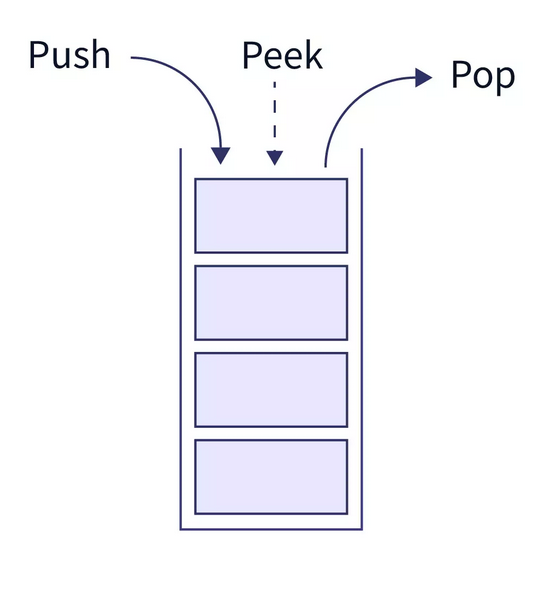
\includegraphics[width=0.5\textwidth]{stack}
            \caption{Source: \url{https://www.scaler.in/stack-operations/}}
        \end{figure}

    \end{columns}
\end{frame}

\begin{frame}{Stacks}{Operationer}
    \begin{columns}
        \column{.3\textwidth}
        \begin{minipage}{\textwidth}
            \scriptsize
            \uncover<1-3>{%
                \begin{tcolorbox}
                    
                    \vspace{-\abovedisplayskip}
                    \begin{codebox}
                        \Procname{$\proc{Stack-Empty}(S)$}
                        \li \If $\attrib{S}{top} \isequal 0$
                            \Then
                        \li     \Return True
                        \li \Else \Return False
                    \end{codebox}
                \end{tcolorbox}
            }

            \uncover<2->{%
                \begin{tcolorbox}
                    
                    \vspace{-\abovedisplayskip}
                    \begin{codebox}
                        \Procname{$\proc{Push}(S,x)$}
                        \li \If $\attrib{S}{top} \isequal \attrib{S}{size}$
                            \Then
                        \li \Error "overflow"
                        \li \Else
                        \li $\attrib{S}{top} \gets \attrib{S}{top} + 1$
                        \li $S[\attrib{S}{top}] \gets x$
                    \end{codebox}
                \end{tcolorbox}
            }

            \uncover<3->{%
                \begin{tcolorbox}
                    
                    \vspace{-\abovedisplayskip}
                    \begin{codebox}
                        \Procname{$\proc{Pop}(S)$}
                        \li \If $\proc{Stack-Empty}(S)$
                            \Then
                        \li \Error "underflow"
                        \li \Else
                        \li $\attrib{S}{top} \gets \attrib{S}{top} - 1$
                        \li \Return $S[\attrib{S}{top} + 1]$
                    \end{codebox}
                \end{tcolorbox}
            }
        \end{minipage}
    
        \column{.39\textwidth}

        \only<4->{Eksempel:}

        \begin{itemize}
            \small
            \item<4-> Vi har stacken $S$ med $\attrib{S}{top} == 4$
            \item<5-> Vi kalder \proc{Push}($S, 17$) og $\proc{Push}(S,3)$
            \item<6-> Nu har vi $\attrib{S}{top} == 6$
            \item<7-> Vi kalder $\proc{Pop}(S)$
            \item<8-> Kaldet returnerer 3 og sætter $\attrib{S}{top} = 5$
            \item<9-> Bemærk at \alert{elementet stadig er i arrayet!}
        \end{itemize}

        \column{.3\textwidth}
        \begin{figure}[h]
            \centering
            \uncover<4->{%
                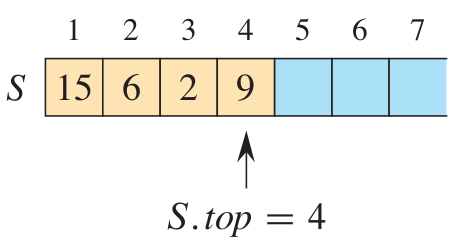
\includegraphics[width=0.8\textwidth]{stack-example/stack-a}
            }
            \uncover<5->{%
                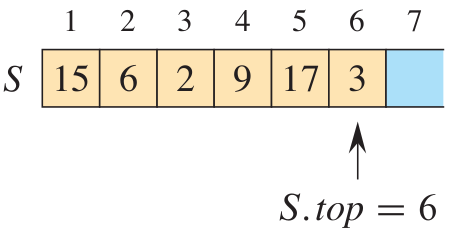
\includegraphics[width=0.8\textwidth]{stack-example/stack-b}
            }
            \uncover<7->{%
                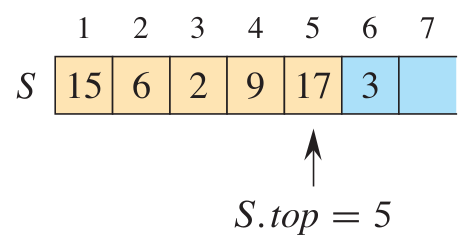
\includegraphics[width=0.8\textwidth]{stack-example/stack-c}
            }
        \end{figure}

    \end{columns}
\end{frame}

\begin{frame}{Queues}{First in, first out}
    En anden klassisk datastruktur er en \alert{queue}, altså en kø. Her følger
    vi \alert{FIFO}-princippet: `First In, First Out'.

    \begin{columns}
        \column{.6\textwidth}
        \begin{itemize}
            \item Insertion og deletion kalder vi henholdsvis \alert{Enqueue} og
                \alert{Dequeue}
            \item For en queue med $n-1$ pladser bruger vi et array $Q[1:n]$
            \item $Q.head$ angiver indexet på det `forreste' element i køen, men
                $Q.tail$ angiver, hvor det næste element skal indsættes
            \item Vi implementerer vores queue med \alert{wrap-around}: dvs.\
                hvis $\attrib{Q}{tail} \isequal \attrib{Q}{size}$ efter vi har
                indsat et element sætter vi $\attrib{Q}{tail} \gets 1$
        \end{itemize}
    
        \column{.4\textwidth}
        \begin{figure}[h]
            \centering
            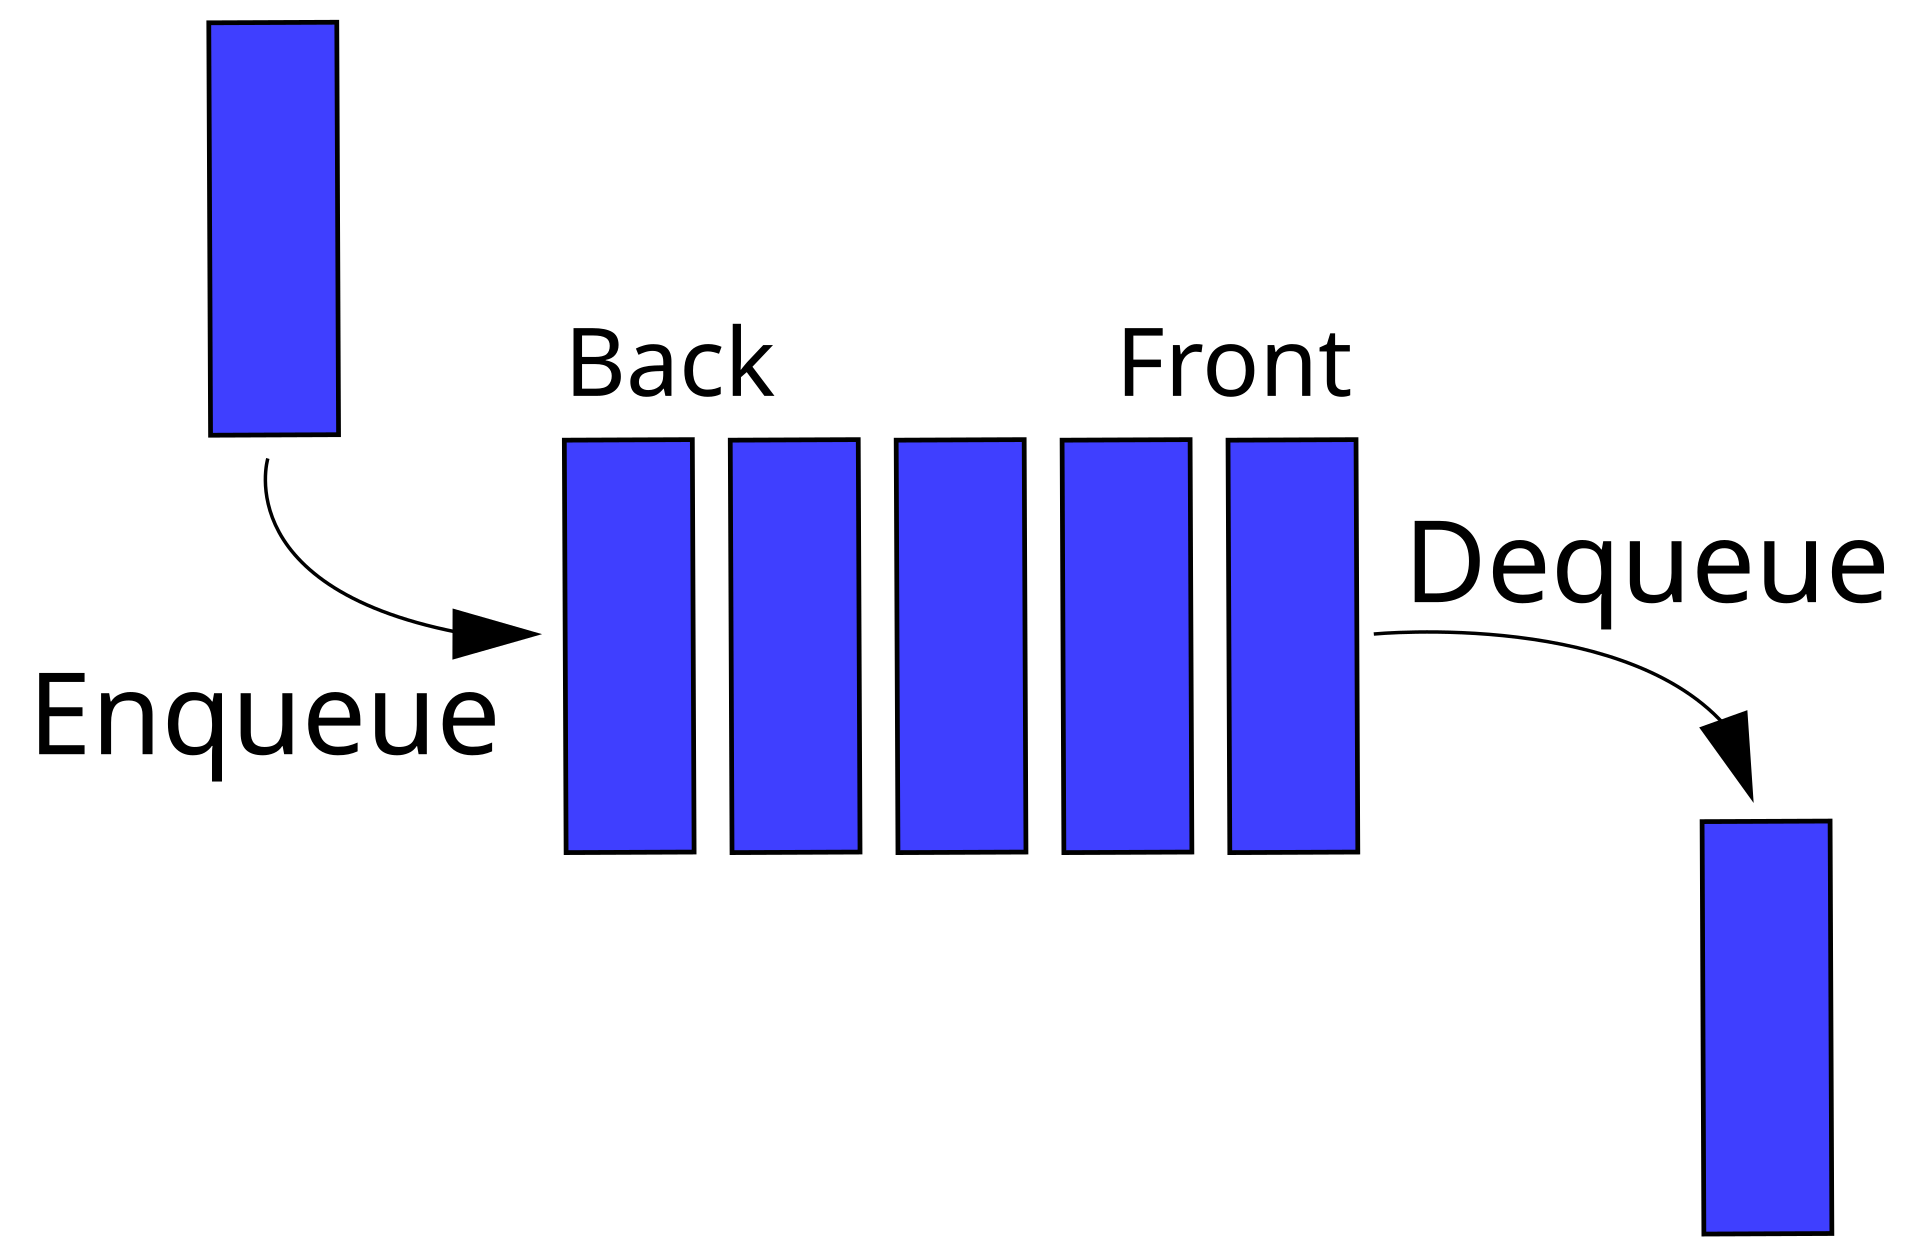
\includegraphics[width=0.8\textwidth]{queue}
            \caption{Source: Wikipedia}
        \end{figure}
    \end{columns}
\end{frame}

\begin{frame}{Queues}{Operationer}
    \begin{columns}
        \column{.35\textwidth}
        \begin{minipage}{\textwidth}
            \scriptsize
            \uncover<1->{%
                \begin{tcolorbox}
                    
                    \vspace{-\abovedisplayskip}
                    \begin{codebox}
                        \Procname{$\proc{Enqueue}(Q, x)$}
                        \li $Q[\attrib{Q}{tail}] \gets x$
                        \li \If $\attrib{Q}{tail} \isequal \attrib{Q}{size}$
                            \Then
                        \li     $\attrib{Q}{tail} \gets 1$
                        \li \Else
                                $\attrib{Q}{tail} \gets \attrib{Q}{tail} + 1$
                            \End
                    \end{codebox}
                \end{tcolorbox}
            }

            \uncover<2->{%
                \begin{tcolorbox}
                    
                    \vspace{-\abovedisplayskip}
                    \begin{codebox}
                        \Procname{$\proc{Dequeue}(Q)$}
                        \li $x \gets Q[\attrib{Q}{head}]$
                        \li \If $\attrib{Q}{head} \isequal \attrib{Q}{size}$
                            \Then
                        \li     $\attrib{Q}{head} \gets 1$
                        \li \Else
                                $\attrib{Q}{head} \gets \attrib{Q}{head} + 1$
                            \End
                        \li \Return $x$
                    \end{codebox}
                \end{tcolorbox}
            }
        \end{minipage}
    
        \column{.35\textwidth}
        \begin{itemize}
            \footnotesize
            \item<3-> Vi har en queue med 5 elementer, hvor $\attrib{Q}{head}$ peger
                på indeks 7 og $\attrib{Q}{tail}$ på indeks 12
            \item<4-> Nu kalder vi $\proc{Enqueue}(Q,17)$, $\proc{Enqueue}(Q,3)$ og
                $\proc{Enqueue}(Q,5)$ (bemærk \alert{wrap-around}!)
            \item<5-> Endelig kalder vi $\proc{Dequeue}(Q)$ som returnerer værdien
                15 og inkrementerer $\attrib{Q}{head}$
        \end{itemize}

        \column{.3\textwidth}
        \begin{figure}[h]
            \centering
            \only<3->{%
                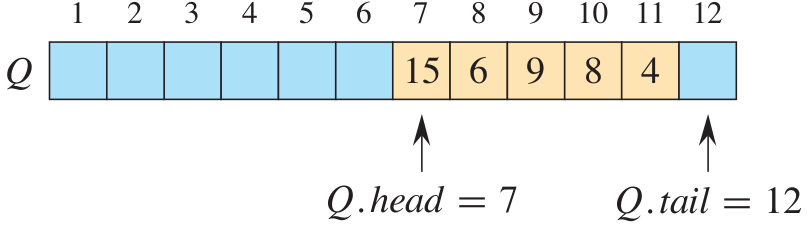
\includegraphics[width=0.95\textwidth]{queue-example/queue-a}
            }
            \only<4->{%
                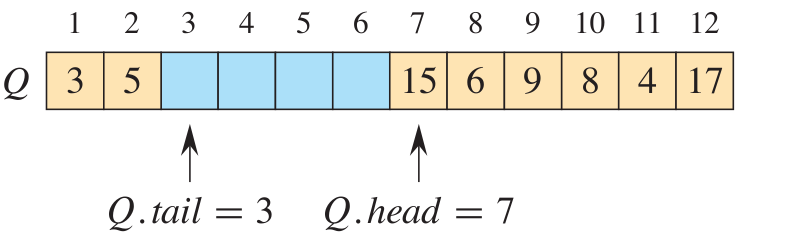
\includegraphics[width=0.95\textwidth]{queue-example/queue-b}
            }
            \only<5->{%
                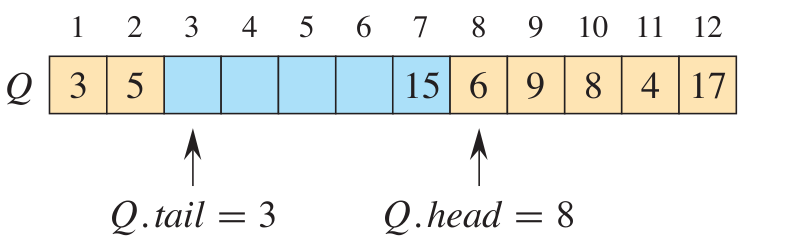
\includegraphics[width=0.95\textwidth]{queue-example/queue-c}
            }
        \end{figure}

    \end{columns}
\end{frame}


\begin{frame}{Linked lists}{`Hægtede' lister!}
    Den sidste af de basale datastruktur for nu er såkalde \alert{linked lists}.
    Dette er en måde at implemntere dynamiske sekvenser på uden brug af arrays.

    \begin{itemize}[<+->]
        \item Hvert element i en linked list $L$ er et \alert{objekt} $x$ med følgende
            attributter:
            \begin{itemize}
                \item $\attrib{x}{key}$ indeholder selve værdien af elementet
                \item $\attrib{x}{next}$ er en pointer til næste element i listen
                \item $\attrib{x}{prev}$ er en pointer til forrige element i
                    listen (kun for \alert{doubly linked lists})
            \end{itemize}
        \item Selve listen har en enkelt attribut $\attrib{L}{head}$ som peger
            på første element i listen
        \item Hvis $\attrib{L}{head} \isequal \const{nil}$ er listen tom
        \item Hvis $\attrib{x}{next} \isequal \const{nil}$ er $x$ sidste element i
            listen
        \item Bemærk at vi ikke behøver beslutte på forhånd, hvor stor en linked
            liste skal være (modsat et array)!
    \end{itemize}

    \centerline{%
        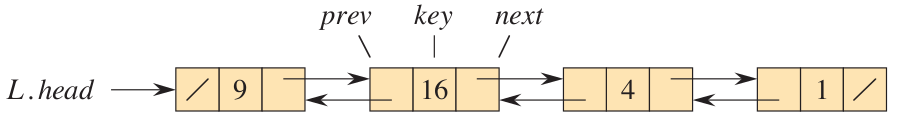
\includegraphics[width=.7\textwidth]{linked-list-example/linked-a}
    }
\end{frame}

\begin{frame}{Linked lists}{Operationer}
    \begin{columns}
        \column{.4\textwidth}
        \small
        
        \begin{block}{$\proc{List-Search}(L,k)$}

            \vspace{-\abovedisplayskip}
            \begin{codebox}
                \li $x \gets \attrib{L}{head}$
                \li \While $x \neq \const{NIL}$ and $\attrib{x}{key} \neq k$
                    \Do
                \li     $x \gets \attrib{x}{next}$
                    \End
                \li \Return $x$
            \end{codebox}
        \end{block}

        \column{.6\textwidth}

        \begin{itemize}[<+->]
            \item \proc{List-Search} tager en liste $L$ og en værdi $k$ som
                input
            \item Finder det første element i listen med nøglen $k$
            \item Returnerer en pointer til dette element ($\const{NIL}$ hvis
                der ikke findes sådan et element)
            \item Hvilken worst-case køretid har $\proc{List-Search}$?
                \begin{itemize}
                    \item Da vi i værste fald skal alle $n$ elementer igennem er
                        køretiden $\Theta(n)$
                \end{itemize}
        \end{itemize}

    \end{columns}

\end{frame}

\begin{frame}{Linked lists}{Prepend og insert}

    \begin{columns}
        \column{.4\textwidth}

        \only<1,2,3,7->{%
            \begin{block}{$\proc{List-Prepend}(L,x)$}

                \vspace{-\abovedisplayskip}
                \begin{codebox}
                    \li $\attrib{x}{next} \gets \attrib{L}{head}$
                    \li $\attrib{x}{prev} \gets \const{NIL}$
                    \li \If $\attrib{L}{head} \neq \const{NIL}$
                        \Then
                    \li     $\attrib{\attrib{L}{head}}{prev} \gets x$
                        \End
                    \li $\attrib{L}{head} \gets x$
                \end{codebox}
            \end{block}
        }
    
        \only<4->{%
            \begin{block}{$\proc{List-Insert}(x,y)$}

                \vspace{-\abovedisplayskip}
                \begin{codebox}
                    \li $\attrib{x}{next} \gets \attrib{y}{next}$
                    \li $\attrib{x}{prev} \gets y$
                    \li \If $\attrib{y}{next} \neq \const{NIL}$
                        \Then
                    \li     $\attrib{\attrib{y}{next}}{prev} \gets x$
                        \End
                    \li $\attrib{y}{next} \gets x$
                \end{codebox}
            \end{block}
        }
    
        \column{.6\textwidth}

        \only<-3>{%
            \begin{itemize}[<+->]
                \item \proc{List-Prepend} tager en liste $L$ og et element $x$ som
                    input
                \item Elementet $x$ indsættes som det første i listen
                \item $\attrib{L}{head}$ skal opdateres og pointers fra det gamle
                    $\attrib{L}{head}$ skal overføres til $x$
            \end{itemize}
        }

        \only<4-6>{%
            \begin{itemize}
                \item<4-> \proc{List-Insert} tager to elementer $x$ og $y$ som input
                \item<5-> Element $x$ indsættes umiddelbart efter $y$ i listen
                \item<6-> Pointers fra $y$ skal overføres til $x$, og $\attrib{x}{next}$
                    skal pege på $y$
            \end{itemize}
        }

        \only<7->{%
            \begin{itemize}
                \item<7-> Bemærk at begge procedurer bevarer den interne rækkefølge
                    af de eksisterende elementer
                \item<8-> Hvilken køretid har de to funktioner?
                    \begin{itemize}
                        \item<9-> Begge er konstante $\Theta(1)$ operationer, da vi
                            kun skal opdatere pointers
                    \end{itemize}
                \item<10-> Hvad ville det kræve at implementere samme funktionalitet
                    i et array?
                    \begin{itemize}
                        \item<11-> Alle elementer efter det indsatte ville skulle
                            flyttes en plads `opad' --- $\Theta(n)$ i worst
                            case!
                        \item<12-> Og måske ville vi være nødt til at kopiere alt
                            over i et nyt, større array
                    \end{itemize}
            \end{itemize}
        }

    \end{columns}

    % \only<-3>{%
        \vspace{\abovedisplayskip}
        \begin{figure}[h]
            \centering
            \includegraphics<-3>[width=0.8\textwidth]{linked-list-example/linked-prepend}
            \includegraphics<4-6>[width=0.8\textwidth]{linked-list-example/linked-insert}
        \end{figure}
    % }
\end{frame}

\begin{frame}{Linked lists}{Deletion}
    \begin{columns}
        \column{.4\textwidth}
        \small
        
        \begin{block}{$\proc{List-Delete}(L,x)$}

            \vspace{-\abovedisplayskip}
            \begin{codebox}
                \li \If $\attrib{x}{next} \neq \const{NIL}$
                    \Then
                \li     $\attrib{\attrib{x}{prev}}{next} \gets \attrib{x}{next}$
                \li \Else
                        $\attrib{L}{head} \gets \attrib{x}{next}$
                    \End
                \li \If $\attrib{x}{next} \neq \const{NIL}$
                    \Then
                \li     $\attrib{\attrib{x}{next}}{prev} \gets \attrib{x}{next}$
                    \End
            \end{codebox}
        \end{block}

        \column{.6\textwidth}

        \begin{itemize}[<+->]
            \item \proc{List-Delete} tager en liste $L$ og et element $x$ som
                input
            \item Sletter $x$ fra listen og opdaterer pointers
            \item Kører også i $\Theta(1)$
                \begin{itemize}
                    \item Medmindre man lige skal finde elementet først\ldots
                \end{itemize}
        \end{itemize}

    \end{columns}

    \vspace{\abovedisplayskip}
    \begin{figure}[h]
        \centering
        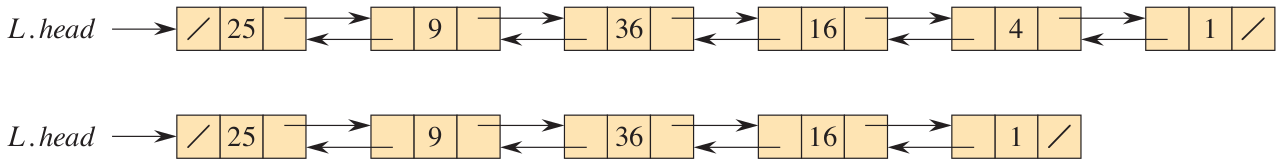
\includegraphics[width=0.8\textwidth]{linked-list-example/linked-delete}
    \end{figure}

\end{frame}


\section{Heaps}

\begin{frame}{Heaps}{En lidt mindre basal datastruktur}
    Nu hvor vi har set en række meget simple datastrukturer kaster vi os over en
    marginalt mere avanceret størrelse: et (binært) \alert{heap}.

    \begin{columns}
        \column{.6\textwidth}
        \only<-5>{%
            \begin{itemize}
                \item<1-> Vi repræsenterer et heap med plads til $n$ elementer med
                    et array $A[1:n]$, men det egentlige antal elementer angives
                    med attributten $\attrib{A}{heap-size}$
                \item<2-> Et heap kan ses som et \alert{næsten komplet} træ,
                    hvor alle niveauer er fyldt ud, pånær måske det sidste som
                    dog skal være fyldt ud fra `venstre' mod `højre'
                \item<3-> Vi siger, at et element på plads $A[i]$ er
                    \alert{parent node} (`forældreknude') for elementerne på
                    plads $A[2i]$ og $A[(2i+1]$, som dermed er venstre og højre
                    barn
                \item<4-> En knude har en `højde' (\alert{height}) svarende til
                    antal kanter på den længste vej fra roden til knuden. Højden
                    på hele heapet er højden på roden, og da et heap er et
                    (næsten) komplet binært træ er dets højde\ldots
                    \uncover<5->{$\Theta(\log n)$}
            \end{itemize}
        }

        \only<6->{%
            \begin{block}
                
                \vspace{-\abovedisplayskip}
                \begin{codebox}
                    \Procname{$\proc{Parent}(i)$}
                    \li \Return $\lfloor i/2 \rfloor$
                \end{codebox}

                \begin{codebox}
                    \Procname{$\proc{Left}(i)$}
                    \li \Return $2i$
                \end{codebox}

                \begin{codebox}
                    \Procname{$\proc{Right}(i)$}
                    \li \Return $2i + 1$
                \end{codebox}
            \end{block}
        }
    
        \column{.4\textwidth}
        \begin{figure}[h]
            \centering
            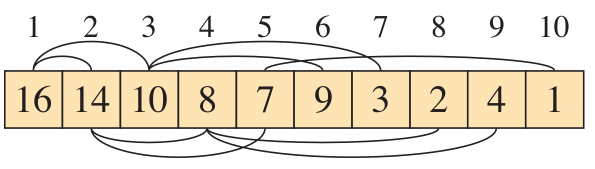
\includegraphics[width=0.8\textwidth]{heaps/array}
            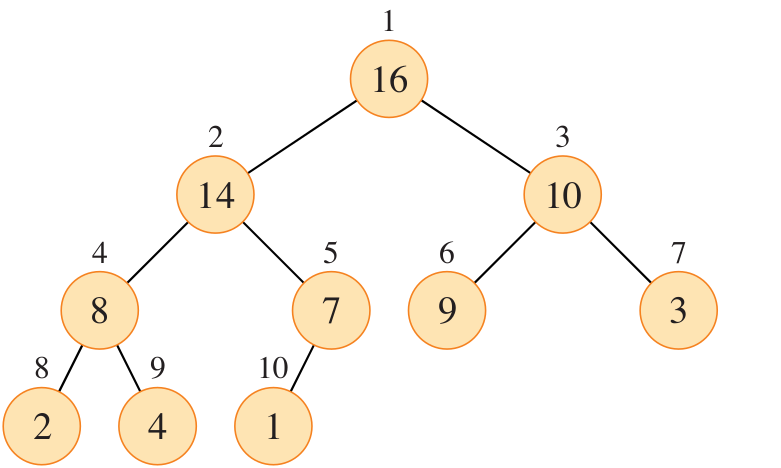
\includegraphics[width=0.8\textwidth]{heaps/tree}
        \end{figure}
    \end{columns}
\end{frame}


\begin{frame}{Heaps}{Heap-property}
    Der er to forskellige slags heaps, som vi kalder hhv. \alert{Max-Heaps} og
    \alert{Min-Heaps}. Hver slags skal opfylde deres respektive
    \alert{heap-property}:

    \begin{block}{Max-Heap property}
        For alle knuder $i > 1$ gælder $A[\proc{Parent}(i)] \geq A[i]$
    \end{block}

    \pause
    \begin{block}{Max-Heap property}
        For alle knuder $i > 1$ gælder $A[\proc{Parent}(i)] \leq A[i]$
    \end{block}

    \pause
    Forskellen er minimial, så for nemheds skyld arbejder vi eksklusivt med
    Max-Heaps.
\end{frame}


\section{Exercises}

\section{Operationer på heaps}

\begin{frame}{Operationer på heaps}{Max-Heapify og Build-Max-Heap}
    Der er to grundlæggende operationer, der knytter sig til heaps:

    \pause
    \begin{itemize}
        \item $\proc{Max-Heapify}(A, i)$ sikrer, at (max-)heap-egenskaben
            opretholdes i træet med rod i $A[i]$
            \pause
        \item $\proc{Build-Max-Heap}(A)$ tager et arbitrært array $A$ og
            konverterer det til et (max-)heap
    \end{itemize}
\end{frame}

\begin{frame}[t]{Operationer på heaps}{Max-Heapify}
    Vi starter med at se på \proc{Max-Heapify}.

    \begin{columns}
        \column{.5\textwidth}
        \only<1>{%
            \begin{itemize}
                \item Formålet er at opretholde max-heap egenskaben
                \item Inputtet er et array $A$ og et index $i$, hvor
                    \proc{Left}($i$) og $\proc{Right}(i)$ er max-heaps, men hvor
                    $A[i]$ \alert{måske} er mindre end $\proc{Left}(i)$ og
                    $\proc{Right}(i)$
                \item Outputtet er det omorganiserede array, der nu overholder
                    max-heap egenskaben i $A[i]$
            \end{itemize}
        }
        
        \only<2->{%
            \begin{itemize}
                \item<2-> Vi starter med at sammenligne $A[i]$ med
                    $A[\proc{Left}(i)]$ og $A[\proc{Right}(i)]$ for at finde ud
                    af, hvilken der er størst
                \item<3-> Så lader vi $A[i]$ `synke' ned i træet ved at bytte det ud
                    med det største af sine børn
                \item<4-> Vi fortsætter rekursivt til $A[i]$ enten er størst eller
                    et blad
            \end{itemize}
        }

        \column{.5\textwidth}
        \begin{figure}[h]
            \centering
            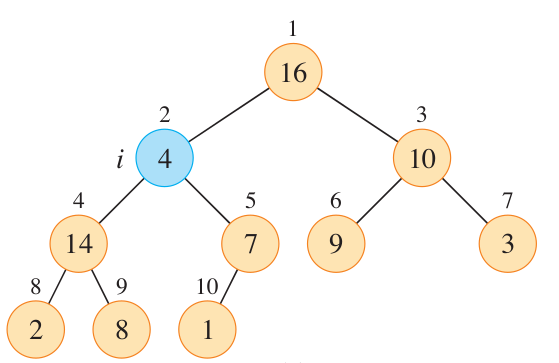
\includegraphics[width=0.8\textwidth]{heaps/max-heapify-a}
        \end{figure}
    
    \end{columns}
\end{frame}

\begin{frame}{Max-Heapify}{Pseudo-kode}

    \begin{columns}
        \column{.5\textwidth}
        \begin{block}{$\proc{Max-Heapify}(A, i)$}
            
            \vspace{-\abovedisplayskip}
            \begin{codebox}
                \li $l \gets \proc{Left}(i)$
                \li $r \gets \proc{Right}(i)$
                
                \li \alertline<2>\If $l \leq \attrib{A}{heap-size}$ and $A[l] > A[i]$
                    \Then
                \li     \alertline<3>$\id{largest} \gets l$
                \li \Else 
                        \alertline<3>$\id{largest} \gets i$
                    \End
                \li \alertline<4>\If $r \leq \attrib{A}{heap-size}$ and $A[r] > A[largest]$
                    \Then
                \li     \alertline<4>$\id{largest} \gets r$
                    \End
                
                \li \alertline<5>\If $\id{largest} \neq i$
                    \Then
                \li     \alertline<5>exchange $A[i]$ with $A[\id{largest}]$
                \li     \alertline<5>$\proc{Max-Heapify}(A, \id{largest})$
                    \End
            \end{codebox}
        \end{block}
    
        \column{.5\textwidth}
        \begin{figure}[h]
            \centering
            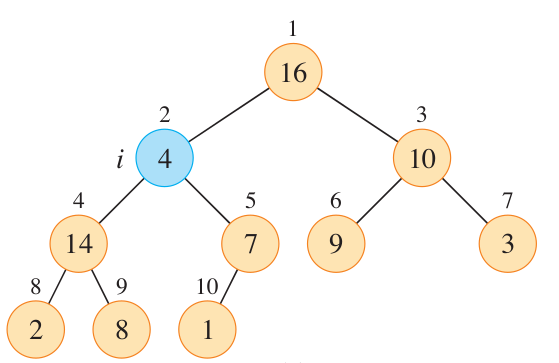
\includegraphics[width=0.5\textwidth]{heaps/max-heapify-a}
        \end{figure}

        \begin{itemize}
            \item<2-> Tjek om venstre barn er i heapet og om det er større end $A[i]$
            \item<3-> Gem hvadend der er størst af $A[i]$ og $A[\proc{Left}(i)]$ i
                variablen $\id{largest}$
            \item<4-> Tjek om højre barn er i heapet og om det er større end
                $\id{largest}$ (og opdater evt $\id{largest}$)
            \item<5-> Hvis det ikke er $A[i]$, der er størst, byt $A[i]$ ud med
                $A[\id{largest}]$ og kald rekursivt
        \end{itemize}
    \end{columns}
    
\end{frame}


\begin{frame}{Max-Heapify}{Eksempel}
    \begin{figure}[h]
        \centering
        \uncover<1->{%
            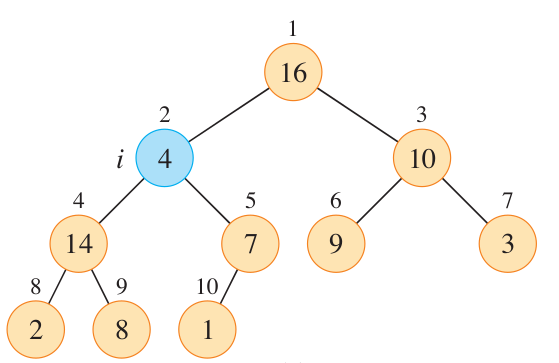
\includegraphics[width=0.3\textwidth]{heaps/max-heapify-a}
        }
        \uncover<2->{%
            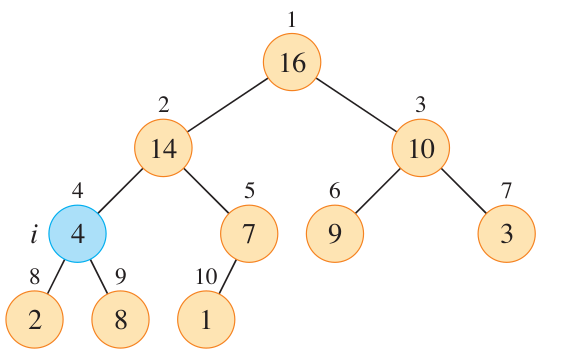
\includegraphics[width=0.3\textwidth]{heaps/max-heapify-b}
        }
        \uncover<3->{%
            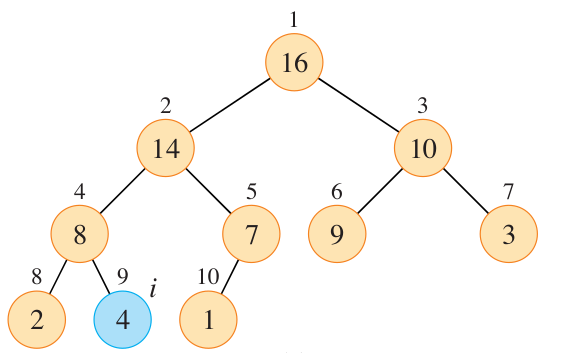
\includegraphics[width=0.3\textwidth]{heaps/max-heapify-c}
        }
    \end{figure}

    \begin{itemize}
        \item<1-> Vi har kaldt $\proc{Max-Heapify}(A,2)$
        \item<2-> $A[2] = 4$ hvilket er mindre end begge børn, så vi bytter
            med det største barn, $A[4]$, og kalder $\proc{Max-Heapify}(A,4)$
        \item<3-> Nu har vi $A[4] = 4$, hvilket er større end det venstre
            barn men mindre end det højre. Vi bytter dem og kalder
            $\proc{Max-Heapify}(A,9)$
        \item<4-> $A[9]$ har ingen børn, så rekursionen slutter nu, og max-heap
            egenskaben er overholdt
    \end{itemize}
\end{frame}

\begin{frame}{Max-Heapify}{Tidsanalyse}
    \begin{columns}
        \column{.5\textwidth}
        \begin{itemize}
            \item<1-> Linie 1-9 er\ldots \only<2->{$\Theta(1)$}
            \item<3-> Hvad med linie 10?
                \begin{itemize}
                    \item<4-> Worst case er, at nederste niveau i træet er halvt
                        fuldt (hvorfor?) --- i så fald har det største sub-træ
                        maks $2n/3$ knuder
                    \item<5-> Dermed er størrelsen af sub-problemet i worst-case
                        $T(2n/3)$
                \end{itemize}
            \item<6-> Vi får altså en rekursion på formen $T(n) = T(2n/3) +
                \Theta(1)$
        \end{itemize}
    
        \column{.5\textwidth}
        \begin{block}{$\proc{Max-Heapify}(A, i)$}
            
            \vspace{-\abovedisplayskip}
            \begin{codebox}
                \li $l \gets \proc{Left}(i)$
                \li $r \gets \proc{Right}(i)$
                
                \li \If $l \leq \attrib{A}{heap-size}$ and $A[l] > A[i]$
                    \Then
                \li     $\id{largest} \gets l$
                \li \Else 
                        $\id{largest} \gets i$
                    \End
                \li \If $r \leq \attrib{A}{heap-size}$ and $A[r] > A[largest]$
                    \Then
                \li     $\id{largest} \gets r$
                    \End
                
                \li \If $\id{largest} \neq i$
                    \Then
                \li     exchange $A[i]$ with $A[\id{largest}]$
                \li     $\proc{Max-Heapify}(A, \id{largest})$
                    \End
            \end{codebox}
        \end{block}
    \end{columns}
\end{frame}


\begin{frame}{Bonus-analyse: Træstruktur}{Worst case størrelse af barn}
    \begin{itemize}
        \small
        \only<-6>{%
            \item<1-> Først, bemærk at det værste split vil være, hvis det ene
                sub-træ er komplet med højde $h$ og det andet komplet med højde
                $h-1$
            \item<2-> Et komplet binært træ med $n$ knuder vil have $k$ `interne knuder'
                og præcis $k+1$ blade (hvorfor?) --- altså er $n = 2k + 1$
            \item<3-> Lad os sige, at det store sub-træ har $2k + 1$ knuder,
                mens det lille, der mangler det sidste niveau af $k + 1$ blade,
                kun har $k$ knuder
            \item<4-> Forældreknuden må således have $n = 1 + (2k + 1) + k = 3k +
                2$ knuder
            \item<5-> Det kan vi omskrive, så vi på højresiden får størrelsen af
                det store sub-træ:
                \begin{align*}
                    &n = 3k + 2 \\
                    \implies \, & \frac{n}{3}= k + \frac{2}{3} \\
                    \implies \, & \frac{2n}{3}= 2k + \frac{4}{3} \\
                    \implies \, & \frac{2n}{3} - \frac{1}{3} = 2k + 1
                \end{align*}
            \item<6-> Altså er $\frac{2n}{3}$ et upper bound på antal knuder i
                et subtræ til et træ med størrelse $n$
        }
    \end{itemize}
\end{frame}


\begin{frame}{Max-Heapify}{Tidsanalyse}
    Så altså\ldots Sub-problemet i det rekursive kald i \proc{Max-Hepify} har i
    værste fald en størrelse på $2n/3$ mens resten er konstant. Kan vi bruge
    master method så? \pause \alert{Ja!}

    \pause

    \begin{itemize}
        \item Vi har $T(n) = T(2n/3) + \Theta(1)$
        \item Dermed: $a = \uncover<4->{3/2}$, $b = \uncover<5->{1}$ og $f(n) =
            \uncover<6->{\Theta(1)}$
        \item<7-> Vi indsætter og forenkler: $n^{\log_{3/2} 1} = n^{0} = 1$
        \item<8-> Vi sammenligner med $f(n)$:
            \begin{align*}
                       &O(n^{0-\epsilon}) \\
                f(n)=\,&\Theta(n^0 \log^{k} n) \\
                       &\Omega(n^{0+\epsilon})
            \end{align*}
        \item<9-> Dette er \alert{case 2} i teoremet, når vi vælger $k=0$, hvilket
            giver os en køretid $T(n) = \Theta(n^0 \log^{k+1} n) = \Theta(\log
            n)$
    \end{itemize}

\end{frame}


\begin{frame}{Build-Max-Heap}{Nu bygger vi et heap!}
    Den næste operation, vi ser på, har det simple formål at konstruere et heap
    ud fra et uorganiseret array $A$.

    \begin{columns}
        \column{.6\textwidth}
        \begin{itemize}[<+->]
            \small
            \item Bemærk først, at den sidste halvdel af $A$ kan betragtes som
                blade i træet og er dermed trivielt korrekte max-heaps (ie.\
                overholder heap-egenskaben)
            \item Dermed skal vi bare kalde \proc{Max-Heapify} på elementerne
                fra plads $n/2$ og ned til 1 for at have håndhævet
                heap-egenskaben på hele arrayet
                \begin{itemize}
                    \item Husk at \proc{Max-Heapify} kaldt på index $i$
                        forventer, at $\proc{Left}(i)$ og $\proc{Right}(i)$
                        overholder heap-egenskaben
                \end{itemize}
            \item Køretiden for linie 2 er $O(n)$ og vi har lige vist at
                \proc{Max-Hepify} er i $\Theta(\log n)$ --- altså en samlet
                køretid på $O(n \log n)$
                \begin{itemize}
                    \item Dog\ldots Med lidt snilde kan man faktisk udlede et
                        strammere bound på \alert{$\Theta(n)$} --- se CLRS 6.3
                \end{itemize}
        \end{itemize}
    
        \column{.4\textwidth}
        \begin{block}{$\proc{Build-Max-Heap}(A,n)$}

            \vspace{-\abovedisplayskip}
            \begin{codebox}
                \li $\attrib{A}{heap-size} \gets n$
                \li \For $i \gets \lfloor n/2 \rfloor$ \Downto $1$ 
                \li     \Do
                            $\proc{Max-Heapify}(A,i)$
                        \End
            \end{codebox}
        \end{block}
    \end{columns}
\end{frame}

\begin{frame}{Build-Max-Heap}{Eksempel}
    Vi kalder proceduren på inputtet $A = \langle 4, 1, 3, 2, 16, 9, 10, 14, 8,
    7  \rangle$.

    \begin{figure}[h]
        \centering
        \uncover<1->{%
            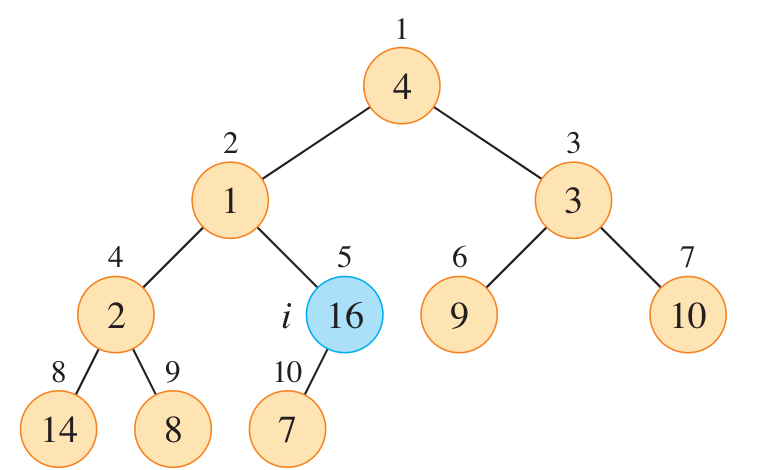
\includegraphics[width=0.3\textwidth]{heaps/build-heap-a}
        }
        \uncover<2->{%
            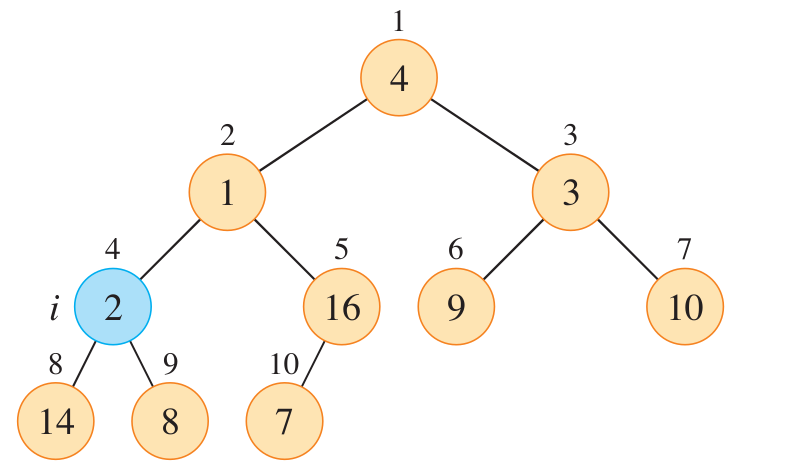
\includegraphics[width=0.3\textwidth]{heaps/build-heap-b}
        }
        \uncover<3->{%
            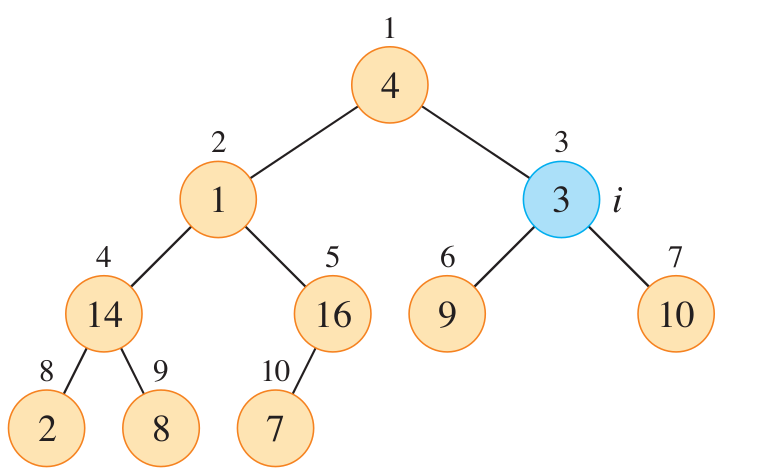
\includegraphics[width=0.3\textwidth]{heaps/build-heap-c}
        }
        \uncover<4->{%
            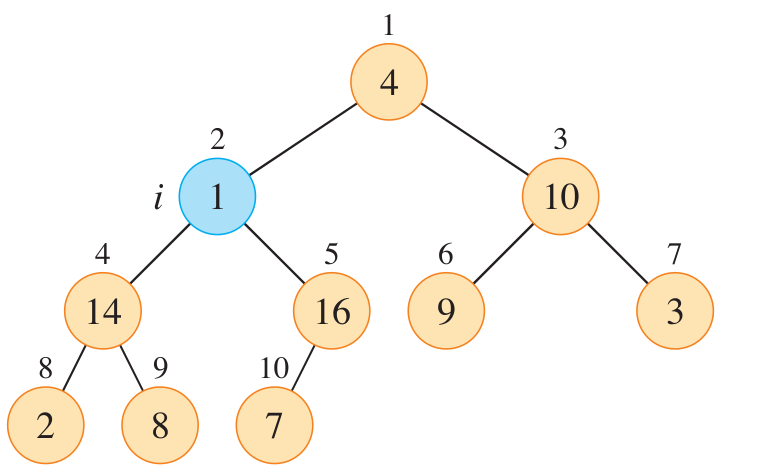
\includegraphics[width=0.3\textwidth]{heaps/build-heap-d}
        }
        \uncover<5->{%
            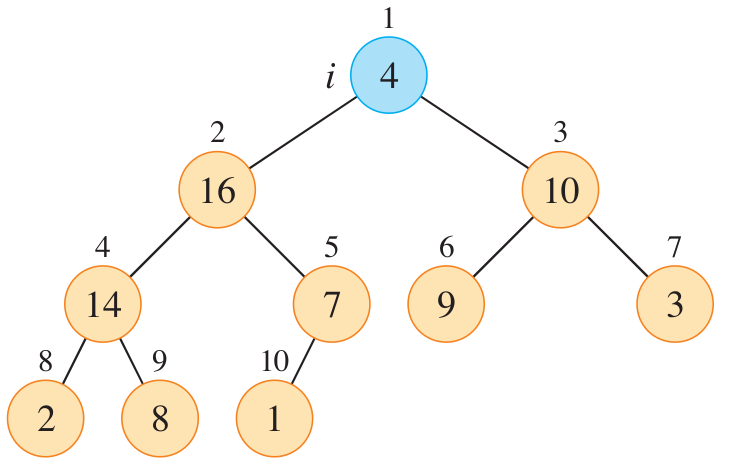
\includegraphics[width=0.3\textwidth]{heaps/build-heap-e}
        }
        \uncover<6->{%
            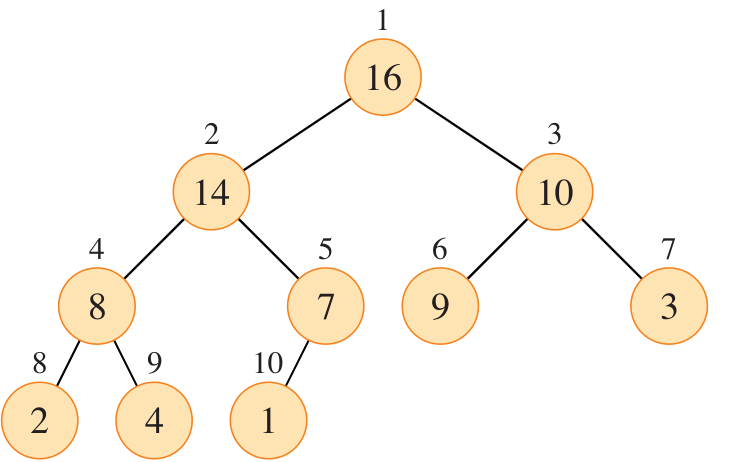
\includegraphics[width=0.3\textwidth]{heaps/build-heap-f}
        }
    \end{figure}

\end{frame}


\section{Heapsort}

\begin{frame}{Heapsort}{Sort of simpelt}
    Nu da vi har \proc{Max-Heapify} og \proc{Build-Max-Heap}, som er to hurtige
    operationer, kan I så forestille jer, hvordan vi kan kombinere de to til en
    sorteringsalgoritme?

    \begin{columns}
        \column{.55\textwidth}
        \begin{itemize}
            \small
            \item<2-> Vi skal sortere $A$, så vi starter med at konvertere det til
                et max-heap
            \item<3-> Nu ved vi, at første element er det største --- altså skal det
                stå sidst i det sorterede array
            \item<4-> Vi bytter derfor det første og sidste element (som er et blad)
                med hinanden og gør \attrib{A}{heap-size} en mindre
            \item<5-> Så kalder vi \proc{Max-Heapify} på det nye forreste element,
                og genopretter dermed heap-egenskaben
            \item<6-> Dette fortsætter vi med, indtil vi har været hele arrayet
                igennem --- til sidst er heapet tomt men arrayet sorteret i
                stigende rækkefølge!
            \item<7-> Kompleksitet?
        \end{itemize}
    
        \column{.45\textwidth}
        \begin{block}{$\proc{Heapsort}(A,n)$}
            
            \vspace{-\abovedisplayskip}
            \begin{codebox}
                \li $\proc{Build-Max-Heap}(A,n)$
                \li \For $i \gets n$ \Downto $2$
                \li     \Do
                            exchange $A[1]$ with $A[i]$
                \li         $\attrib{A}{heap-size} \gets \attrib{A}{heap-size}
                            - 1$
                \li         $\proc{Max-Heapify}(A,1)$         
                        \End
            \end{codebox}
        \end{block}
    \end{columns}
\end{frame}

\begin{frame}{Heapsort}{Sort of simpelt}
    Vi vil sortere sekvensen $A = \langle 4, 1, 3, 2, 16, 9, 10, 14, 8, 7
    \rangle$:

    \begin{columns}
        \column{.75\textwidth}
        
        \begin{figure}[h]
            \centering
            \uncover<2->{%
                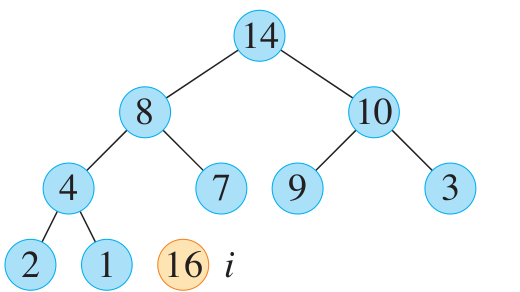
\includegraphics[width=0.3\textwidth]{heaps/heapsort-b}
            }
            \uncover<3->{%
                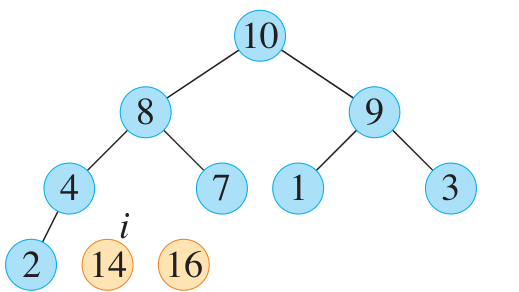
\includegraphics[width=0.3\textwidth]{heaps/heapsort-c}
            }
            \uncover<4->{%
                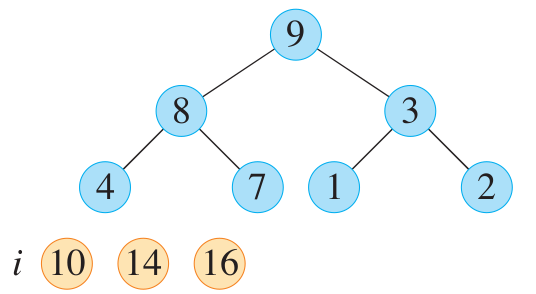
\includegraphics[width=0.3\textwidth]{heaps/heapsort-d}
            }
            \uncover<5->{%
                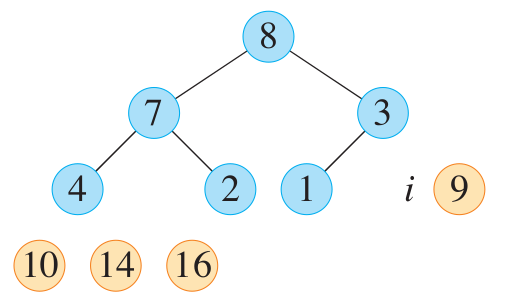
\includegraphics[width=0.3\textwidth]{heaps/heapsort-e}
            }
            \uncover<6->{%
                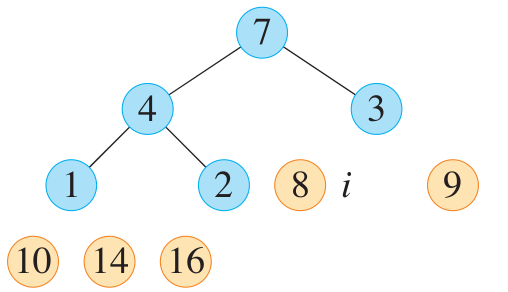
\includegraphics[width=0.3\textwidth]{heaps/heapsort-f}
            }
            \uncover<7->{%
                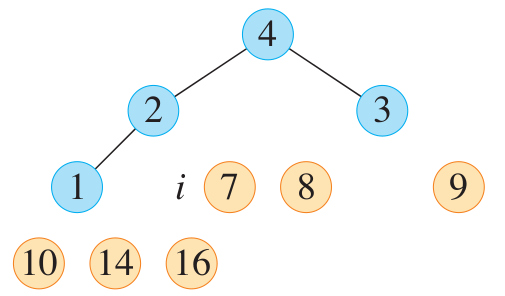
\includegraphics[width=0.3\textwidth]{heaps/heapsort-g}
            }
            \uncover<8->{%
                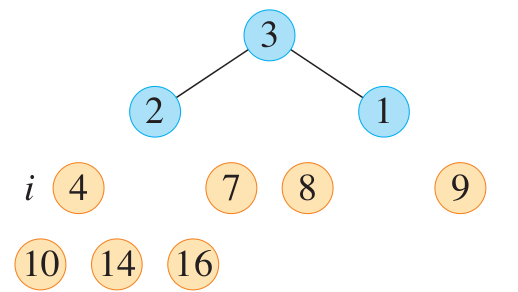
\includegraphics[width=0.3\textwidth]{heaps/heapsort-h}
            }
            \uncover<9->{%
                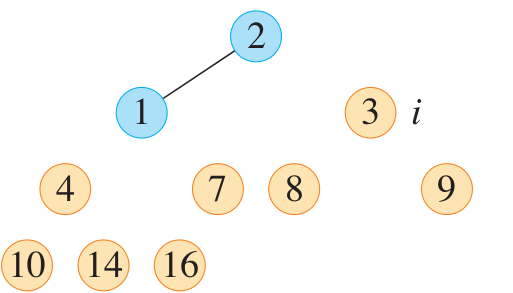
\includegraphics[width=0.3\textwidth]{heaps/heapsort-i}
            }
            \uncover<10->{%
                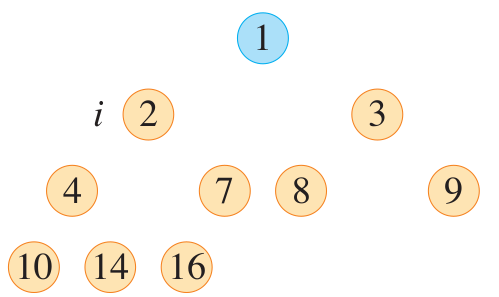
\includegraphics[width=0.3\textwidth]{heaps/heapsort-j}
            }
        \end{figure}
    
        \column{.25\textwidth}
        \begin{block}{$\proc{Heapsort}(A,n)$}
            \scriptsize
            
            \vspace{-\abovedisplayskip}
            \begin{codebox}
                \li $\proc{Build-Max-Heap}(A,n)$
                \li \For $i \gets n$ \Downto $2$
                \li     \Do
                            swap $A[1]$ and $A[i]$
                \li         $\attrib{A}{heap-size}--$
                      
                \li         $\proc{Max-Heapify}(A,1)$         
                        \End
            \end{codebox}
        \end{block}

        \footnotesize
        \begin{figure}[h]
            \centering
            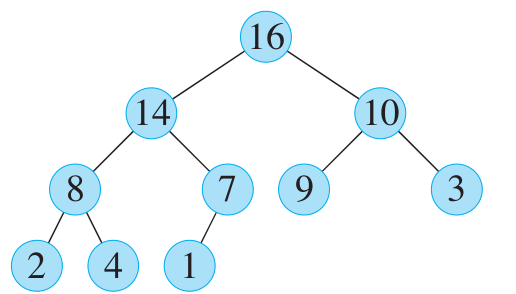
\includegraphics[width=0.9\textwidth]{heaps/heapsort-a}
        \end{figure}

        Current status $A = \langle
        \only<1>{16}\only<2>{14}\only<3>{10}\only<4>{9}\only<5>{8}\only<6>{7}\only<7>{4}\only<8>{3}\only<9>{2}\only<10->{1},
        \only<1>{14}\only<2-4>{8}\only<5>{7}\only<6>{4}\only<7-8>{2}\only<9>{1}\only<10->{2},
        \only<1-2>{10}\only<3>{9}\only<4-7>{3}\only<8>{1}\only<9->{3},
        \only<1>{8}\only<2-5>{4}\only<6-7>{1}\only<8->{4},
        \only<1-4>{7}\only<5-6>{2}\only<7->{7},
        \only<1-2>{9}\only<3-5>{1}\only<6->{8},
        \only<1-3>{3}\only<4>{2}\only<5->{9},
        \only<1-3>{2}\only<4->{10},
        \only<1>{4}\only<2>{1}\only<3->{14},
        \only<1>{1}\only<2->{16}
        \rangle$

    \end{columns}
\end{frame}

\section{Priority Queues}

\begin{frame}{Priority queues}{Prioriterede køer}
    Heapsort er god, fordi den både kører i $\Theta(n \log n)$ tid og sorter
    in-place, og dermed kun kræver $\Theta(1)$ ekstra plads. Men i praksis er
    quicksort typisk hurtigere\ldots Heaps hart dog et andet trick i ærmet,
    nemlig \alert{priority queues}!

    \begin{itemize}
        \item Abstrakt datastruktur, der understøtter operationerne
            $\proc{Insert}$, $\proc{Extract-Maximum}$ og $\proc{Maximum}$
        \item En dynamisk kø, hvor rækkefølgen ikke er bestemt af
            indsættelsesrækkefølgen men af en given \alert{key}
        \item Forestil jer en skadestue, hvor ham med den forstuvede finger
            måske dukkede op først, men hende med en punkteret lunge alligevel
            skal forrest i køen (eller I kan forestille jer noget mindre
            makabert, såsom en job scheduler i en computer eller noget andet
            kedeligt)
    \end{itemize}
\end{frame}

\begin{frame}{Priority queues}{Operationer}
    Vi kigger først på $\proc{Insert}$-proceduren.

    \begin{columns}
        \column{.5\textwidth}
        \small
        \begin{itemize}[<+->]
            \item Vi tager som input et heap $A$ og et element $x$, vi vil
                indsætte
            \item Vi øger $\attrib{A}{heap-size}$ med 1 for at gøre plads
                (tjekker selvfølgelig, at $\attrib{A}{heap-size} <
                \attrib{A}{length}$)
            \item Vi indsætter $x$ bagerst i heapet og lader det `svømme' opad,
                ved at bytte det ud med sin forældrer, så længe det er større
            \item Kompleksitet?
                \begin{itemize}
                    \item Siden hver iteration af while-løkken flytter elementet
                        et niveau op i træet, så udgør højden af træet et tight
                        bound --- $\Theta(\log n)$
                \end{itemize}
        \end{itemize}
    
        \column{.5\textwidth}
        \begin{block}{$\proc{Insert}(A,x)$}
            \small
            
            \vspace{-\abovedisplayskip}
            \begin{codebox}
                \Procname{$\proc{}$}
                \li $\attrib{A}{heap-size} \gets \attrib{A}{heap-size} + 1$
                \li $A[\attrib{A}{heap-size}] \gets x$
                \li $\id{i} \gets \attrib{A}{heap-size}$
                \li \While $i > 1$ and $A[\attrib{\proc{Parent}(i)}{key}] <
                    \attrib{A[i]}{key}$
                \li \Do
                        exchange $A[i]$ with $A[\proc{Parent}(i)]$
                \li     $i \gets \proc{Parent}(i)$
                    \End
            \end{codebox}
        \end{block}
    \end{columns}
\end{frame}

\begin{frame}{Priority queues}{The CLRS way}
    Bemærk, at CLRS gør det en smule anderledes. Det er essentielt set det
    samme, så det er fint, hvis I bare forstår $\proc{Insert}$  på sidste slide.

    \begin{figure}[h]
        \centering
        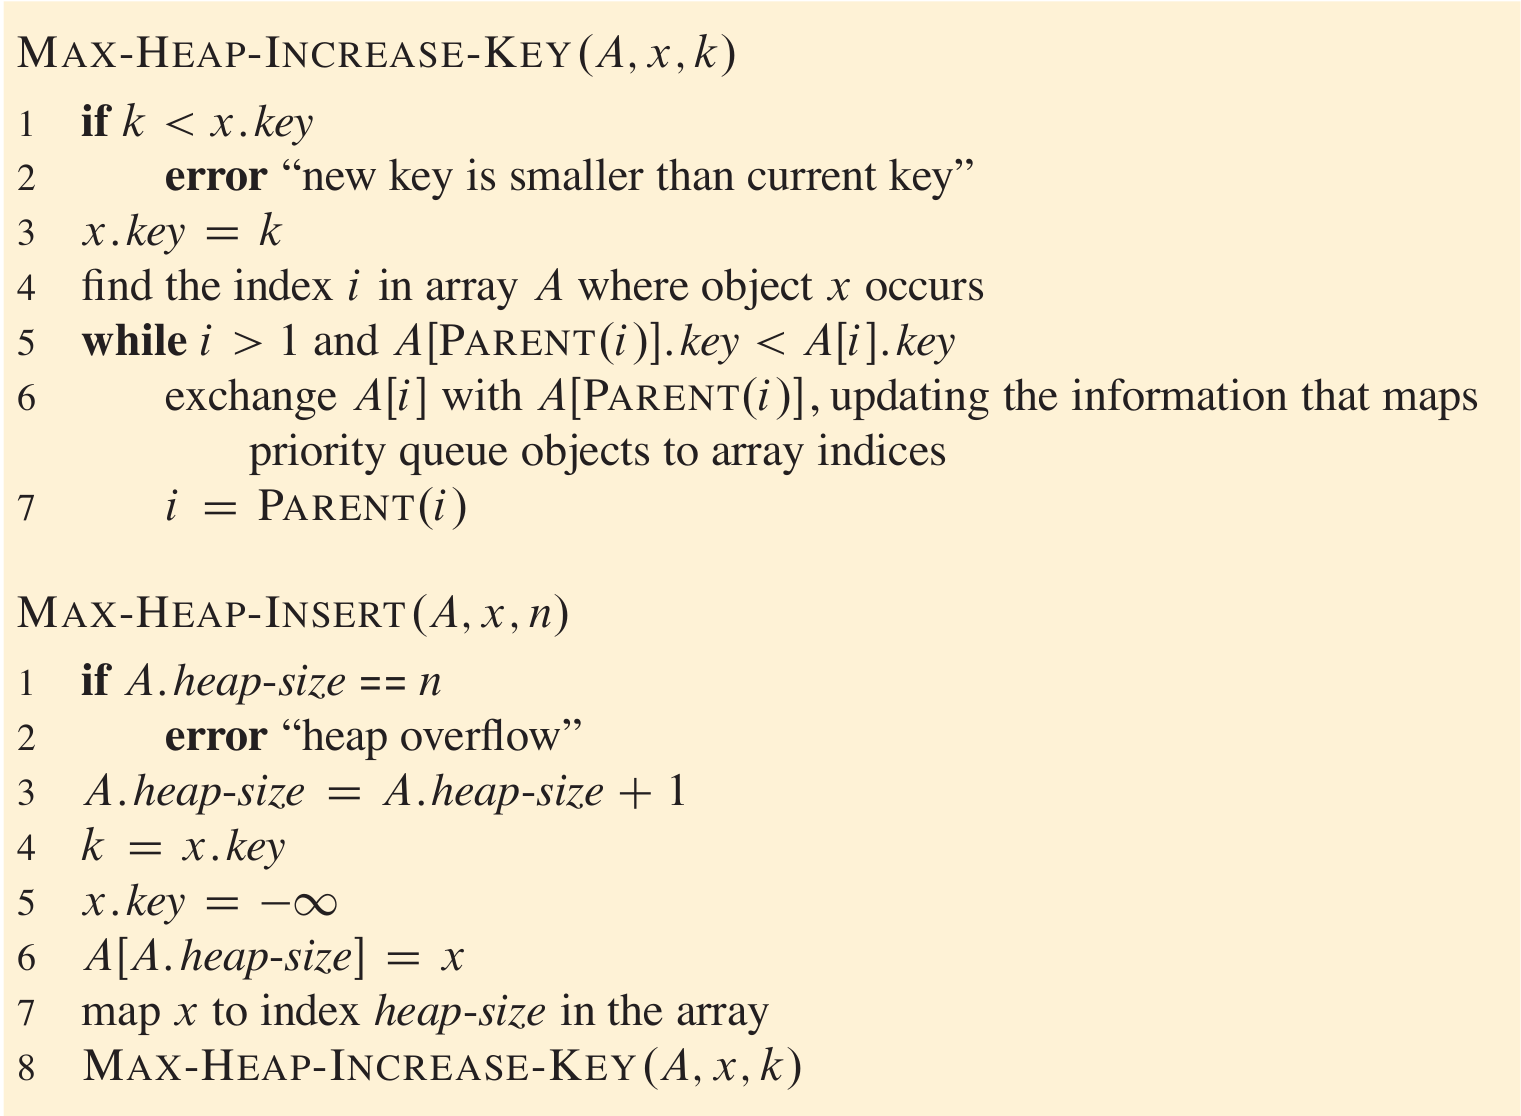
\includegraphics[width=0.6\textwidth]{heaps/max-heap-insert-clrs}
    \end{figure}
\end{frame}

\begin{frame}{Priority queues}{Extract-Maximum}
    Sidst men ikke mindst, så ser vi på, hvordan vi kan slette det største
    element fra en priority queue.

    \begin{columns}
        \column{.5\textwidth}
        \begin{itemize}
            \small
            \item Vi gemmer det største element (som også er det første element)
                i en variable $\id{max}$
            \item Vi flytter det sidste element frem til at stå på index 1
            \item Vi sænker $\attrib{A}{heap-size}$
            \item Vi kalder $\proc{Max-Heapify}(A,1)$ og reetablerer dermed
                heap-egenskaben
            \item Slutteligt returnerer vi $\id{max}$
            \item Og glædeligt nok er denne operation også $\Theta(\log n)$!
        \end{itemize}
    
        \column{.5\textwidth}
        \begin{block}{$\proc{Heap-Extract-Max}(A)$}
            
            \vspace{-\abovedisplayskip}
            \begin{codebox}
                \li $\id{max} \gets A[1]$
                \li $A[1] \gets A[\attrib{A}{heap-size}]$
                \li $\attrib{A}{heap-size} \gets \attrib{A}{heap-size} - 1$
                \li $\proc{Max-Heapify}(A,1)$
                \li \Return $\id{max}$
            \end{codebox}
        \end{block}
    \end{columns}
\end{frame}


\begin{frame}{Slut på forelæsning 4}{Puh!}
    Endelig\ldots
\end{frame}





\begin{frame}{Dagens temaer}{Opsummering}
    \begin{itemize}
        \small
        \item<1-> Vi har mødt basale datastrukturer som \alert{stacks},
            \alert{queues} og \alert{linked lists}
            \begin{itemize}
                \item Stacks følger LIFO (`last in, first out')
                \item Queues følger FIFI (`first in, first out')
                \item Linked lists erstatter array-fundamentet med pointers fra
                    hvert element til det næste (og til det forrige, hvis det er
                    en \alert{doubly linked list})
            \end{itemize}
        \item<2-> Vi har mødt \alert{heaps} og lært
            \begin{itemize}
                \item at et heap, der kan fortolkes som et binært træ
                \item at et \alert{max-heap} skal overholde
                    \alert{heap-egenskaben}: `For alle $i > 1$ gælder
                    $A[\proc{Parent}(i)] \geq A[i]$'
                \item at vi med \alert{$\proc{Max-Heapify}$} i $\Theta(\log n)$
                    tid kan re-etablere heap-egenskaben i en knude $A[i]$, så
                    længe $\proc{Left}(i)$ og $\proc{Right}(i)$ er rødder i
                    træer, der overholder den
                \item at vi kan bygge et heap i $\Theta(n)$ fra et uorganiseret
                    array med \alert{$\proc{Build-Max-Heap}$}
            \end{itemize}
        \item<3-> Vi har også set på to applikationer for heaps
            \begin{itemize}
                \item Vi kan sortere in-place og i $\Theta(n \log n)$ med
                    \alert{heapsort}, der udnytter heap-strukturen og de
                    logaritmiske operationer
                \item Vi kan implementere en \alert{priority queue} med heaps og
                    understøtte insertion og deletion i $\Theta(\log n)$ tid
            \end{itemize}
    \end{itemize}
\end{frame}


\begin{frame}{Tak for i dag!}{Flere exercises..}

    Den bedste måde ikke at snyde sig selv på er lave exercises!

    \begin{figure}[h]
        \centering
        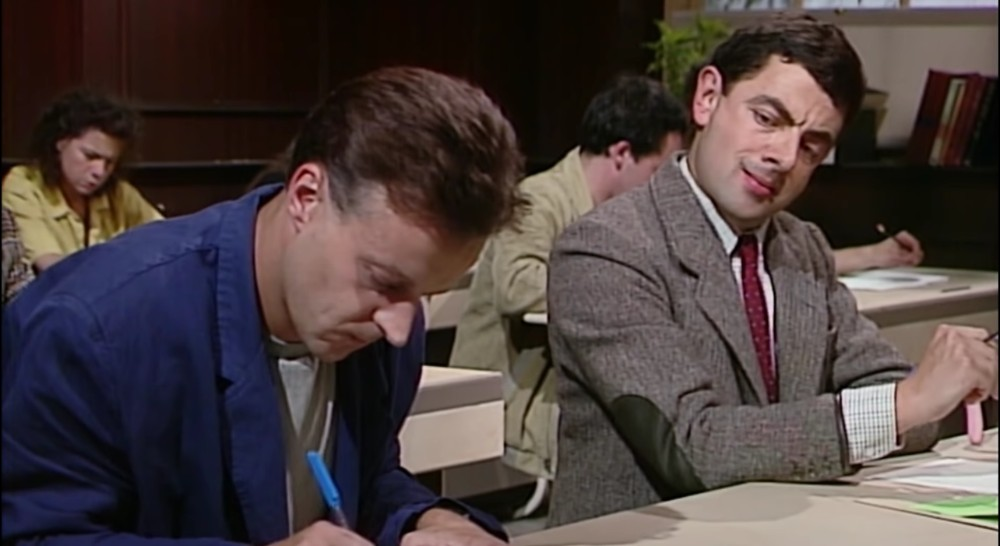
\includegraphics[width=0.8\textwidth]{exercises}
    \end{figure}
    
\end{frame}



\end{document}


